\chapter{Point de vue developpeur}

\section{Documentation}
Notre Javadoc des différents plugins est disponible ici \cite{doc}
\clearpage

\section{Conception}
	\subsection{Architecture et classes}
	Dans cette partie nous détaillerons l'architecture de notre application, à travers ses différents points d'extensions.
	\begin{figure}[!htbp]
	  \centering
	  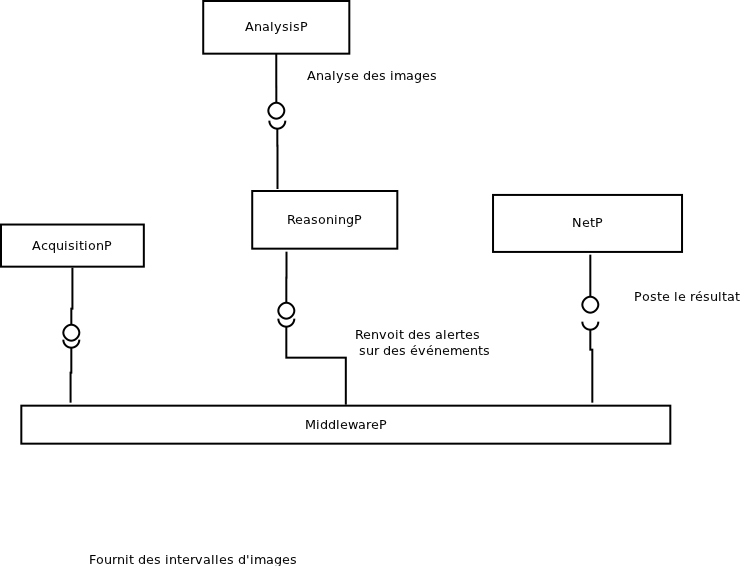
\includegraphics[scale=0.50]{img/archi}
	  \caption{Architecture de l'outil}
	  \label{fig:archi}
	\end{figure}


		\paragraph{Architecture}
		qsdqs
		\paragraph{Acquisition}
		Le plugin Acquisition consiste à récupérer un fichier vidéo et en extraire une image périodiquement. Le plugin répond aux spécifications fournies par l'interface \verb+IFlux+ (cf. Fig \ref{fig:IFlux}).
		\begin{figure}[htbp]
			\centering
			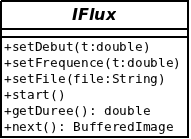
\includegraphics[scale=0.50]{img/IFlux}
			\caption{Interface IFlux}
			\label{fig:IFlux}
		\end{figure}

		Pour pouvoir lancer le plugin il est nécessaire d'appeler au minimum les méthodes suivantes dans cet ordre :
		\begin{enumerate}
			\item{\verb+setFile(file)+} pour fournir le fichier vidéo à analyser.
			\item{\verb+start()+} Cette méthode permet de paramètrer l'aquisition et de charger un player. 
			\item{\verb+next()+} renvoie un \verb+BufferedImage+ et avance dans la vidéo.
		\end{enumerate}

		Les autres méthodes de l'interface IFlux sont :
		\begin{itemize}
			\item{\verb+setDebut(tEnSecondes)+} pour donner l'instant à partir duquel la vidéo sera analysée. Cette méthode doit être lancée avant \verb+start()+ ou alors \verb+start+ est relancée
			\item{\verb+setFrequence(tEnSecondes)+} Le nom de la méthode est trompeuse mais elle permet de donner la période en secondes à laquelle le plugin récupère un image dans la vidéo. La période peut être changée avant ou en cours d'acquisition. Cependant le pointeur sur la prochaine image à acquérir étant déjà défini, le changement de période ne sera effectif qu'à partir du second \verb+next()+
			\item{\verb+getDurée()+} renvoie un le temps en secondes de la vidéo. \verb+start()+ doit avoir été déja lancée.
		\end{itemize}

	Pour effectuer l'acquisition le plugin utilise la librairie JMF qui est malheureusement peu pratique puisqu'elle ne gère qu'un faible nombre de formats vidéo. De plus nous avons pu constater un bug au niveau de la méthode qui renvoie la durée de la vidéo \verb+Player.duration()+; en effet celle-ci renvoie une valeur bien trop grande par rapport à la longueur réelle de la vidéo.

		\paragraph{Reasoning}
			\subparagraph{Analyseur d'image}
				Afin de détecter des situations dites "interessantes" telles que la nuit, la présence d'une ou plusieurs personnes, un mouvement particulier, nous proposons un couple de plugin : Reasoning et Analyse. Le plugin Reasoning utilise des informations formelles pour en déduire une situation. Si l'image est sombre pendant un certain temps, il peut en conclure qu'il fait nuit et qu'il n'y a pas de lumières d'allumée. Si une personne se déplace la nuit, c'est peut-être un voleur. Des horaires pourraient être ajoutés pour signaler des déplacements normaux, par exemple un gardien, et tout mouvement non prévu serait signalé.
	Les informations formelles sont détectés par le plugin d'analyse, qui essait de trouver certaines propriétés dans une image. Par exemple, pour affirmer qu'une image est sombre, les canaux de couleurs de chaque pixels sont analysés, et si l'un d'entre eux correspond à une couleur sombre, le pixel est considéré comme sombre. Si 50 des pixels sont sombres, l'algorithme signal que l'image possède cette propriété.
	
	000000 => FFFFFF : RRGGBB => 8 bit pour chaque couleur
			\subparagraph{Image sombre}
				La couleur d'un pixel est composé de 3 canaux: Rouge, bleu, vert. Pour chaque canal, 256 nuances sont possibles (codé de 0 à 255).
				\begin{enumerate}
					\item Pour chaque pixel, obtenir la valeur des trois canaux avec BufferedImage.getRGB(i,j); où i correspond à l'absice et j à l'ordonnée. 
					\item La valeur obtenu par cette méthode est un entier allant de -16775675 à 0 (tout noir à tout blanc), correspondant à la valeur décimale de la chaine Hexadécimal qui représente réellement la couleur. Ce nombre est négatif car le bit de poids fort correspond normalement à l'alpha (le fait que l'image est une couleur transparente ou non).
					\item Pour obtenir la valeur de chaque canal (Rouge, Vert, Bleu) nous décalons les bits en fonction de ceux que nous souhaitons conserver : s'il faut obtenir la valeur du canal correspondant au vert, il faut décaler de 8 bit vers la droite pour supprimer la partie correspondant au bleu, et appliquer un masque pour ne garder que les 8 derniers bits, le canal bleu. Exemple : 0000000001101011000000000 : les 3 canaux + la valeur alpha, l'algorithme applique un décalage de 8 bit vers la droite : 00000000011010110, puis il ne conserve que les 8 derniers : 11010110. Le bleu est donc à 236 (ou EC en hexadecimal).
					\item Après obtention des 3 canaux, si l'un d'entre eux est trop clair, la couleur le sera. Il faut donc les tester, nous avons choisis un palier de "100", après avoir étudier la composition des couleurs, nous considerons que c'est au dessus de ce palier que les couleurs apparaissent comme étant clair.
				\end{enumerate}
				\begin{figure}[!h]
					\centering
					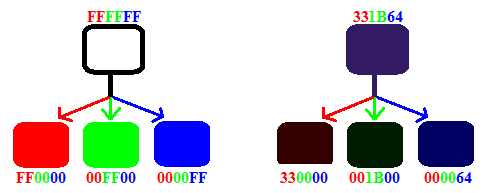
\includegraphics{img/reasoningRGB.png}
					\caption{Exemple de division du blanc à gauche et d'une couleur violette "sombre" à gauche}
					\label{divisionRGB}
				\end{figure}
				
			\subparagraph{Composition de l'image}
					Arbitrairement nous avons choisis de considérer une image comme étant sombre si plus de la moitié de ses pixels le sont.
					
			\subparagraph{Detecteur de presence : Utilisation d'OpenCV}
				Nous n'avons pas développer cet aspect de l'analyse de vidéo/image, mais nos recherches préliminaires nous ont quand même permis d'apprendre certaines choses sur le fonctionnement de la bibliothèque OpenCV : L'image est balayée par un classifieur binaire ("visage" ou "non-visage"), puis les zones où un visage a été détecté sont refondues entre elles afin qu'un même visage ne monopolise pas plusieurs cibles. 
				Pour accèlerer l'algorithme de détection il y a deux méthode :
				\begin{enumerate}
					\item augmenter la taille minimale des cibles à détecter dans l'appel de fonction : dans cette configuration, si on s'éloignes de la caméra, l'algorithme perd la personne, ce n'est donc pas une très bonne idée.
					\item Un moyen plus simple pour accélérer l'algorithme serait de travailler sur une image de résolution plus petite (l'algorithme rétrécit l'image avant de la passer à la fonction) : le calcul de l'image intégrale (qui est effectué en prétraitement dans la fonction) prendra alors beaucoup moins de temps : meilleure idée.
				\end{enumerate}
		
			\subparagraph{Différence de performance}
				Les performances ne vont pas être les mêmes : ce qui est long dans cette fonction, ce n'est pas tant les calculs en eux-mêmes (les classifieurs appliquent des ondelettes de haar, en se servant d'images intégrales pour rendre constante la complexité des calculs, quelle que soit la taille de l'image), mais surtout les pré-traitements.
			
			L'image est redimensionnée plusieurs fois pendant le traitement (c'est un paramètre step, il peut ralentir l'algo s'il est trop fin) de manière à détecter des visages de tailles variées, et à chaque fois une image intégrale est créée (ce qui implique de parcourir tous les pixels de l'image).
			
			Si nous divisons la résolution de l'image de base par 2, en adaptant la taille des cibles minimales, ces pré-traitements prendront 4 fois moins de temps car l'aire à traiter sera divisée par 4. Il est intéressant de faire varier le step pour vérifier son impact sur les performances et trouver un équilibre entre qualité de détection et vitesse d'exécution.
			
				\begin{figure}[!h]
					\centering
					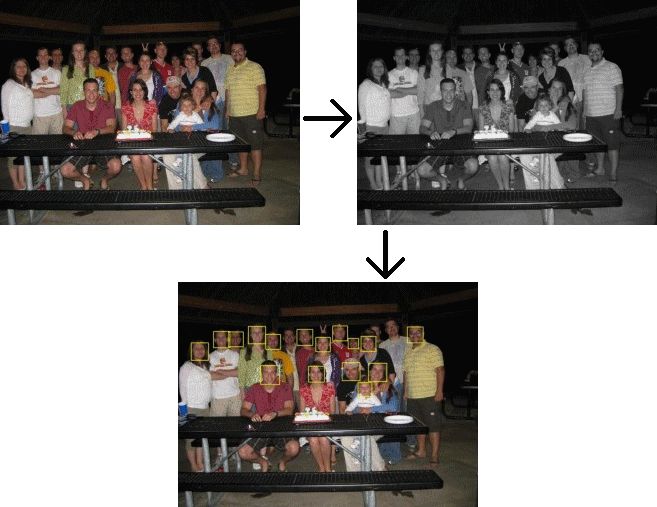
\includegraphics{img/reasoningVisages.png}
					\caption{Image de départ d'une résolution X*Y, elle est passé en X/2 * Y/2 et en nuance de gris, les visages sont detectés, et l'algorithme détermine sur l'image original où sont les visages}
					\label{divisionRGB}
				\end{figure}
			
			\subparagraph{Optimisation}
				Il est préférable que l'image à laquelle on appliques un traitement soit en niveaux de gris. Dans le cas inverse, soit le traitement est appliqué aux 3 canaux (donc 3 fois plus long), soit appliqué a un seul canal (donc moins précis), mais ce n'est pas intéressant car la fonction est prévu pour des images en niveaux de gris.
		\paragraph{NetP}
			Le  NetP est dédié à poster des informations sur un  réseau social ou un blog. Un contributeur de ce point d'extension doit être en mesure de proposer une solution pour chaque action que recquière Middleware. Ces actions sont données dans l'interface \verb+IIformation+ suivante :
			\begin{figure}[!htbp]
				\centering
				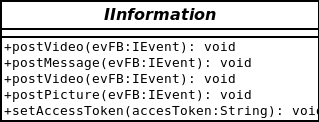
\includegraphics[scale=0.50]{img/iinterface}
				\caption{Interface pour NetP}
				\label{fig:IInterface}
			\end{figure}

			Le contributeur que nous avons implémenté propose d'utiliser le réseau social Facebook et utilise la librairie suivante \cite{restFB}.

\section{Robustesse}
	Bah comme on a mit du JUnit, on est over protected. Et au pire on appelle l'Agence tout risque.
	
\section{Qualité du code}
	Tip top nickel crome. On a tout optimisé a fond, plein de commentaire pour que ce soit compréhensible, bien aéré, bref, perfect.
	
\section{Facilité de mise en oeuvre des extension}
	
